%%%%%%%%%%%%%%%%%%%%%%%%%%%%%%%%%%%%%%%%%%%%%%%%%%%%%%%%%%%%%%%%%%%%%%%%%%%%%%%
% CASE STUDY TEMPLATE - Programming and Problem Solving
% Author: Brendan Shea, PhD
% Course: Programming and Problem Solving
% Rochester Community and Technical College
%%%%%%%%%%%%%%%%%%%%%%%%%%%%%%%%%%%%%%%%%%%%%%%%%%%%%%%%%%%%%%%%%%%%%%%%%%%%%%%

\documentclass[11pt,letterpaper]{article}

%---------- PACKAGES ----------%
\usepackage[margin=1in, headheight=22pt]{geometry}
\usepackage[T1]{fontenc}
\usepackage{xcolor}
\usepackage{tcolorbox}
\usepackage{graphicx}
\usepackage{titlesec}
\usepackage{enumitem}
\usepackage{fancyhdr}
\usepackage{listings}
\usepackage{hyperref}
\usepackage{multicol}
\usepackage{booktabs}
\usepackage{tikz}
\usepackage{float}
\usepackage{amssymb}  % For math symbols
\usepackage{pifont}   % For checkmark: \ding{51}

% TikZ libraries
\usetikzlibrary{shapes.geometric, arrows.meta, positioning, calc, backgrounds, fit, matrix, decorations.pathreplacing}

% Load tcolorbox libraries
\tcbuselibrary{skins,breakable,listings,listingsutf8}

%---------- COLOR DEFINITIONS ----------%
\definecolor{csprimary}{HTML}{2C3E50}
\definecolor{cssecondary}{HTML}{E74C3C}
\definecolor{cstertiary}{HTML}{3498DB}
\definecolor{csaccent}{HTML}{27AE60}
\definecolor{cswarm}{HTML}{F39C12}
\definecolor{cslight}{HTML}{ECF0F1}
\definecolor{csdark}{HTML}{1A252F}

% Syntax highlighting colors
\definecolor{codegreen}{HTML}{27AE60}
\definecolor{codepurple}{HTML}{9B59B6}
\definecolor{codeorange}{HTML}{E67E22}
\definecolor{codeblue}{HTML}{3498DB}
\definecolor{codegray}{HTML}{95A5A6}
\definecolor{codestring}{HTML}{E74C3C}
\definecolor{codebg}{HTML}{1E2A38}

%---------- CASE STUDY METADATA ----------%
\newcommand{\cstitle}{When Algorithms Decide}
\newcommand{\cssubtitle}{Fairness, Bias, and the Ethics of Automated Decisions}
\newcommand{\csauthor}{Brendan Shea, PhD}
\newcommand{\cscourse}{Programming and Problem Solving}
\newcommand{\csinstitution}{Rochester Community and Technical College}
\newcommand{\csdate}{\today}

%---------- LISTINGS CONFIGURATION ----------%
\lstdefinestyle{basestyle}{
    backgroundcolor=\color{codebg},
    basicstyle=\ttfamily\small\color{white},
    breakatwhitespace=false,
    breaklines=true,
    captionpos=b,
    keepspaces=true,
    showspaces=false,
    showstringspaces=false,
    showtabs=false,
    tabsize=4,
    frame=none,
    xleftmargin=4mm,
    xrightmargin=4mm,
    aboveskip=0pt,
    belowskip=0pt,
}

\lstdefinestyle{javastyle}{
    style=basestyle,
    language=Java,
    keywordstyle=\color{codeblue}\bfseries,
    commentstyle=\color{codegray}\itshape,
    stringstyle=\color{codestring},
    morekeywords={String, Scanner, System, var, boolean, Applicant},
}

%---------- CUSTOM ENVIRONMENTS ----------%
\newcommand{\keyterm}[1]{\textbf{\textcolor{cssecondary}{#1}}}

\newtcolorbox{conceptbox}[1][]{
    enhanced,
    colback=cslight,
    colframe=csprimary,
    fonttitle=\bfseries\color{white},
    title=#1,
    attach boxed title to top left={yshift=-2mm, xshift=5mm},
    boxed title style={colback=csprimary},
    breakable
}

\newtcolorbox{historybox}[1][]{
    enhanced,
    colback=codepurple!8,
    colframe=codepurple,
    fonttitle=\bfseries\color{white},
    title=#1,
    attach boxed title to top left={yshift=-2mm, xshift=5mm},
    boxed title style={colback=codepurple},
    breakable
}

\newtcolorbox{casebox}[1][]{
    enhanced,
    colback=cswarm!8,
    colframe=cswarm,
    fonttitle=\bfseries\color{white},
    title=#1,
    attach boxed title to top left={yshift=-2mm, xshift=5mm},
    boxed title style={colback=cswarm},
    breakable
}

\newtcolorbox{codebox}[2][]{
    enhanced,
    colback=codebg,
    colframe=csaccent,
    colupper=white,
    fonttitle=\bfseries\color{white},
    title=#2,
    attach boxed title to top left={yshift=-2mm, xshift=5mm},
    boxed title style={colback=csaccent},
    left=0mm, right=0mm, top=2mm, bottom=2mm,
    boxrule=1pt,
    breakable,
    pad at break=2mm,
    #1
}

\newtcblisting{javacode}[1][]{
    enhanced,
    colback=codebg,
    colframe=csaccent,
    colupper=white,
    fonttitle=\bfseries\color{white},
    title=#1,
    attach boxed title to top left={yshift=-2mm, xshift=5mm},
    boxed title style={colback=csaccent},
    left=0mm, right=0mm, top=2mm, bottom=2mm,
    boxrule=1pt,
    breakable,
    pad at break=2mm,
    listing only,
    listing options={style=javastyle}
}

\newtcolorbox{questionbox}{
    enhanced,
    colback=cswarm!10,
    colframe=cswarm,
    fonttitle=\bfseries\color{white},
    title=Discussion Questions,
    attach boxed title to top center={yshift=-2mm},
    boxed title style={colback=cswarm},
    breakable
}

\newtcolorbox{glossarybox}{
    enhanced,
    colback=cslight,
    colframe=csprimary,
    fonttitle=\bfseries\color{white},
    title=Glossary of Key Terms,
    attach boxed title to top center={yshift=-2mm},
    boxed title style={colback=csprimary},
    breakable
}

%---------- HEADER/FOOTER ----------%
\pagestyle{fancy}
\fancyhf{}
\fancyhead[L]{\small\textcolor{csprimary}{\cscourse}}
\fancyhead[R]{\small\textcolor{csprimary}{Case Study}}
\fancyfoot[C]{\thepage}
\renewcommand{\headrulewidth}{0.4pt}
\renewcommand{\headrule}{\hbox to\headwidth{\color{csprimary}\leaders\hrule height \headrulewidth\hfill}}

%---------- SECTION FORMATTING ----------%
\titleformat{\section}
    {\Large\bfseries\color{csprimary}}
    {\thesection}{1em}{}[\color{cssecondary}\titlerule]
    
\titleformat{\subsection}
    {\large\bfseries\color{cstertiary}}
    {\thesubsection}{1em}{}

%---------- HYPERLINK SETTINGS ----------%
\hypersetup{
    colorlinks=true,
    linkcolor=cstertiary,
    urlcolor=cstertiary
}

%%%%%%%%%%%%%%%%%%%%%%%%%%%%%%%%%%%%%%%%%%%%%%%%%%%%%%%%%%%%%%%%%%%%%%%%%%%%%%%
\begin{document}

%---------- TITLE BLOCK ----------%
\begin{tcolorbox}[
    enhanced,
    colback=csprimary,
    colframe=csprimary,
    arc=0mm,
    left=10mm, right=10mm, top=8mm, bottom=8mm
]
\begin{center}
    {\huge\bfseries\color{white}\cstitle}\\[3mm]
    {\Large\color{cslight}\cssubtitle}\\[5mm]
    \textcolor{cssecondary}{\rule{0.5\textwidth}{1pt}}\\[5mm]
    {\large\color{white}\csauthor}\\[2mm]
    {\normalsize\color{cslight}\cscourse\ $\bullet$ \csinstitution}
\end{center}
\end{tcolorbox}

\vspace{5mm}

%---------- INTRODUCTION ----------%
\section*{Introduction}

Should a computer program decide whether you get a job interview? Whether you're approved for a loan? Whether you're released from jail before your trial? These questions might sound like science fiction, but they describe reality. \keyterm{Algorithms} now make or influence countless decisions that profoundly affect people's lives---often without those people knowing an algorithm was involved.

This case study explores what algorithms are, how they've come to wield such power, and most importantly, what it means for an algorithm to be ``fair.'' As you'll discover, fairness is far more complicated than it first appears. Different definitions of fairness can contradict each other, forcing us to make difficult trade-offs. These aren't just technical problems for computer scientists---they're ethical questions that affect everyone.

\begin{conceptbox}[The Stakes Are Real]
In the United States alone, algorithms influence decisions about who gets hired at major companies, who receives loans, who sees which political advertisements, what news stories appear in your feed, how long criminal sentences should be, and whether patients receive certain medical treatments. Learning to think critically about algorithmic decision-making is no longer optional---it's essential.
\end{conceptbox}

%---------- WHAT IS AN ALGORITHM ----------%
\section{What Is an Algorithm?}

An \keyterm{algorithm} is simply a precise sequence of steps for solving a problem or accomplishing a task. You follow algorithms every day: a recipe is an algorithm for cooking a dish; directions to a friend's house are an algorithm for navigation; the method you learned for long division is an algorithm for arithmetic.

What makes computer algorithms special is that they can be executed automatically, at tremendous speed, on massive amounts of data. A human loan officer might review fifty applications per day; an algorithm can evaluate millions per hour. This scale transforms algorithms from mere tools into systems that shape society.

\begin{javacode}[A Simple Decision Algorithm]
// Should we approve this loan application?
public boolean approveLoan(Applicant app) {
    int score = 0;
    
    // Award points for positive factors
    if (app.creditScore > 700) score += 30;
    if (app.yearsEmployed > 2) score += 20;
    if (app.income > 50000) score += 25;
    if (app.hasCollateral) score += 15;
    
    // Subtract points for risk factors  
    if (app.missedPayments > 0) score -= 20;
    if (app.bankruptcyHistory) score -= 40;
    
    return score >= 50;  // Approve if score meets threshold
}
\end{javacode}

This simple algorithm illustrates key features of algorithmic decision-making. It takes \keyterm{inputs} (data about the applicant), applies \keyterm{rules} (the if-statements that award or subtract points), and produces an \keyterm{output} (approve or deny). The rules encode assumptions about what makes someone creditworthy. But are these assumptions correct? Are they fair?

\subsection{From Rules to Learning}

The loan algorithm above uses rules that humans explicitly wrote. But increasingly, algorithms \textit{learn} their rules from data. \keyterm{Machine learning} algorithms are given many examples (thousands of past loan applications and whether they defaulted) and discover patterns themselves. This can uncover subtle relationships humans might miss---but it can also learn patterns we wouldn't endorse if we knew about them.

\begin{center}
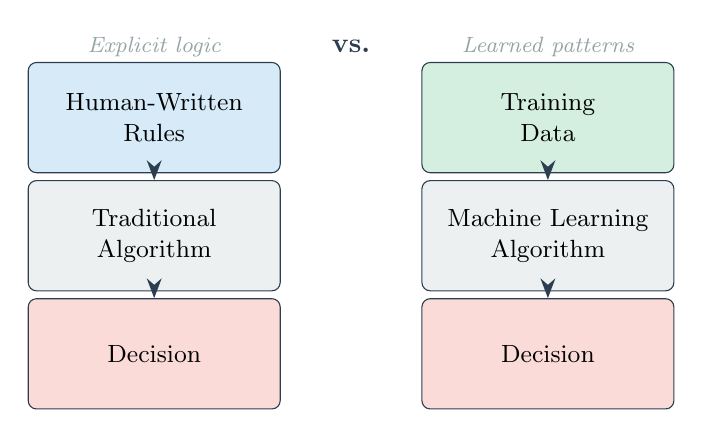
\begin{tikzpicture}[
    box/.style={rectangle, rounded corners=3pt, draw=csprimary, fill=#1, minimum width=32mm, minimum height=14mm, font=\small, align=center},
    arrow/.style={-{Stealth[length=2.5mm]}, thick, color=csprimary}
]

% Traditional algorithm
\node[box=cstertiary!20] (rules) at (0,1.5) {Human-Written\\Rules};
\node[box=cslight] (trad) at (0,0) {Traditional\\Algorithm};
\node[box=cssecondary!20] (out1) at (0,-1.5) {Decision};

\draw[arrow] (rules) -- (trad);
\draw[arrow] (trad) -- (out1);

% ML algorithm
\node[box=csaccent!20] (data) at (5,1.5) {Training\\Data};
\node[box=cslight] (ml) at (5,0) {Machine Learning\\Algorithm};
\node[box=cssecondary!20] (out2) at (5,-1.5) {Decision};

\draw[arrow] (data) -- (ml);
\draw[arrow] (ml) -- (out2);

% Labels
\node[font=\footnotesize\itshape, color=codegray] at (0,2.4) {Explicit logic};
\node[font=\footnotesize\itshape, color=codegray] at (5,2.4) {Learned patterns};

\node[font=\bfseries, color=csprimary] at (2.5,2.4) {vs.};

\end{tikzpicture}
\end{center}

%---------- THE PROBLEM OF BIAS ----------%
\section{The Problem of Bias}

In 2014, Amazon built a machine learning system to review résumés and identify promising job candidates. The algorithm was trained on ten years of hiring data---résumés the company had received and which candidates were ultimately hired. The system learned to predict which new applicants would be successful.

There was just one problem: it learned to penalize résumés that included the word ``women's'' (as in ``women's chess club captain'') and to downgrade graduates of all-women's colleges. Why? Because the training data reflected a decade of hiring in the male-dominated tech industry. The algorithm learned that being male correlated with being hired---not because men were actually better candidates, but because of historical \keyterm{bias} in human decisions.

\begin{casebox}[Case Study: COMPAS and Criminal Justice]
COMPAS (Correctional Offender Management Profiling for Alternative Sanctions) is an algorithm used across the United States to predict whether a defendant will commit future crimes. Judges use these ``risk scores'' when deciding bail, sentencing, and parole.

In 2016, the investigative news organization ProPublica analyzed COMPAS predictions for over 7,000 defendants in Florida. They found that Black defendants were almost twice as likely as white defendants to be incorrectly labeled as high-risk (meaning they were predicted to reoffend but didn't). White defendants, meanwhile, were more likely to be incorrectly labeled as low-risk (meaning they were predicted not to reoffend but did).

The company that makes COMPAS, Northpointe (now Equivant), disputed these findings. They argued their algorithm was fair by a different measure: among defendants who received the same risk score, Black and white defendants reoffended at similar rates.

Both claims were mathematically true. How could the algorithm be simultaneously fair and unfair?
\end{casebox}

The COMPAS controversy reveals something profound: \keyterm{algorithmic fairness} isn't a single concept with a single definition. There are multiple, mathematically incompatible ways to define what ``fair'' means.

%---------- DEFINITIONS OF FAIRNESS ----------%
\section{Competing Definitions of Fairness}

Philosophers, mathematicians, and computer scientists have proposed many definitions of algorithmic fairness. Here are three major approaches:

\subsection{Demographic Parity}

\keyterm{Demographic parity} (also called statistical parity) requires that the algorithm produce positive outcomes at equal rates across different groups. If 30\% of male applicants are hired, then 30\% of female applicants should be hired too.

\begin{javacode}[Testing for Demographic Parity]
// Check if hiring rates are similar across groups
double maleHireRate = (double) malesHired / malesApplied;
double femaleHireRate = (double) femalesHired / femalesApplied;

boolean hasParity = Math.abs(maleHireRate - femaleHireRate) < 0.05;
// True if rates are within 5% of each other
\end{javacode}

The appeal is obvious: equal outcomes suggest equal treatment. But critics argue this definition has problems. What if the applicant pools differ in relevant qualifications? Forcing equal outcomes might mean hiring less-qualified candidates from one group or rejecting more-qualified candidates from another.

\subsection{Equal Accuracy}

\keyterm{Equal accuracy} (sometimes called equalized odds) requires that the algorithm make errors at equal rates across groups. If the algorithm incorrectly rejects 5\% of qualified male applicants, it should also incorrectly reject 5\% of qualified female applicants.

This focuses on the algorithm's \textit{mistakes} rather than its overall outcomes. The intuition is that people shouldn't face a higher burden of proof based on their group membership. A qualified applicant deserves fair consideration regardless of demographic category.

\subsection{Individual Fairness}

\keyterm{Individual fairness} takes a different approach entirely: similar individuals should be treated similarly. Rather than comparing groups, it asks whether two people with nearly identical qualifications receive nearly identical treatment.

\begin{center}
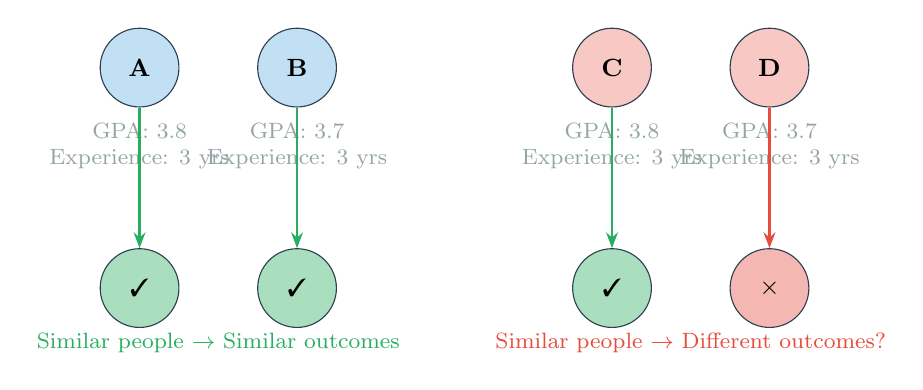
\begin{tikzpicture}[
    person/.style={circle, draw=csprimary, fill=#1, minimum size=10mm, font=\small\bfseries},
    label/.style={font=\footnotesize},
    arrow/.style={-{Stealth[length=2mm]}, thick}
]

% Two similar applicants
\node[person=cstertiary!30] (a1) at (0,0) {A};
\node[person=cstertiary!30] (a2) at (2,0) {B};

\node[label, color=codegray, align=center] at (0,-1) {GPA: 3.8\\Experience: 3 yrs};
\node[label, color=codegray, align=center] at (2,-1) {GPA: 3.7\\Experience: 3 yrs};

% Outcomes
\node[person=csaccent!40] (h1) at (0,-2.8) {\ding{51}};
\node[person=csaccent!40] (h2) at (2,-2.8) {\ding{51}};

\draw[arrow, color=csaccent] (a1) -- (h1);
\draw[arrow, color=csaccent] (a2) -- (h2);

\node[label, color=csaccent] at (1,-3.5) {Similar people $\rightarrow$ Similar outcomes};

% Unfair scenario
\node[person=cssecondary!30] (b1) at (6,0) {C};
\node[person=cssecondary!30] (b2) at (8,0) {D};

\node[label, color=codegray, align=center] at (6,-1) {GPA: 3.8\\Experience: 3 yrs};
\node[label, color=codegray, align=center] at (8,-1) {GPA: 3.7\\Experience: 3 yrs};

\node[person=csaccent!40] (h3) at (6,-2.8) {\ding{51}};
\node[person=cssecondary!40] (h4) at (8,-2.8) {$\times$};

\draw[arrow, color=csaccent] (b1) -- (h3);
\draw[arrow, color=cssecondary] (b2) -- (h4);

\node[label, color=cssecondary] at (7,-3.5) {Similar people $\rightarrow$ Different outcomes?};

\end{tikzpicture}
\end{center}

The challenge with individual fairness is defining ``similar.'' Which characteristics matter? Is someone with a 3.8 GPA and 2 years of experience ``similar'' to someone with a 3.5 GPA and 4 years of experience?

%---------- THE IMPOSSIBILITY THEOREM ----------%
\section{The Impossibility of Perfect Fairness}

Here's the uncomfortable truth that emerged from the COMPAS debate: mathematically, you often \textit{cannot} satisfy multiple fairness definitions simultaneously. This isn't a failure of clever engineering---it's a proven mathematical impossibility.

\begin{historybox}[The Fairness Impossibility Theorems]
In 2016, researchers including Jon Kleinberg, Sendhil Mullainathan, and Manish Raghavan proved that except in special cases, no algorithm can simultaneously achieve:

\begin{enumerate}[leftmargin=*, itemsep=2pt]
    \item \textbf{Calibration}: Among people who receive the same risk score, actual outcomes should be similar across groups.
    \item \textbf{Equal false positive rates}: The rate of incorrectly flagging someone as high-risk should be equal across groups.
    \item \textbf{Equal false negative rates}: The rate of incorrectly missing someone who is high-risk should be equal across groups.
\end{enumerate}

The only exception is when base rates are identical across groups---for instance, if men and women actually defaulted on loans at exactly the same rate. In the real world, base rates often differ (for complex historical and social reasons), making perfect fairness by all measures impossible.
\end{historybox}

This impossibility forces us to make choices. Which type of fairness matters most in a given context? The answer depends on values, not just mathematics. In criminal justice, incorrectly labeling someone as high-risk (a false positive) means they might stay in jail awaiting trial. Incorrectly labeling someone as low-risk (a false negative) means they might commit another crime. Which error is worse? That's an ethical question, not a technical one.

%---------- SOURCES OF BIAS ----------%
\section{Where Does Bias Come From?}

Understanding algorithmic bias requires tracing its sources. Bias can enter at multiple stages:

\subsection{Biased Training Data}

Machine learning algorithms learn from historical data. If that history reflects discrimination, the algorithm learns to discriminate. Amazon's résumé screener learned from a decade of biased hiring. Facial recognition systems trained primarily on light-skinned faces perform worse on darker-skinned faces---not because of any explicit rule, but because the training data was unrepresentative.

\subsection{Biased Problem Framing}

Sometimes the bias is in how we define the problem. Consider an algorithm to predict ``employee success.'' If success is measured by promotions, and promotions have historically been biased, the algorithm optimizes for a biased outcome. The algorithm might work perfectly at its stated goal while perpetuating injustice.

\subsection{Proxy Variables}

Even if we remove protected characteristics like race or gender from the algorithm's inputs, other variables can serve as \keyterm{proxies}. ZIP codes correlate with race due to historical segregation. Names can indicate gender or ethnicity. An algorithm that has never ``seen'' race might still effectively use race through these proxies.

\begin{javacode}[The Proxy Problem]
// This algorithm doesn't use race directly...
public int calculateRiskScore(Applicant app) {
    int score = 50;
    
    // But ZIP code correlates with race
    if (isHighIncomeZipCode(app.zipCode)) score += 15;
    
    // Name patterns correlate with ethnicity
    if (hasCommonDefaultPattern(app.name)) score -= 10;
    
    // Education correlates with family wealth
    if (app.collegeRanking < 50) score += 20;
    
    return score;
}
// ...but it might still produce racially disparate outcomes
\end{javacode}

\subsection{Feedback Loops}

Algorithms can create self-fulfilling prophecies. If a ``predictive policing'' algorithm sends more officers to certain neighborhoods, more arrests occur there, which generates data suggesting those neighborhoods are high-crime, which sends even more officers. The algorithm's predictions become true \textit{because} of the algorithm, not because of underlying reality.

%---------- TRANSPARENCY AND ACCOUNTABILITY ----------%
\section{Transparency and Accountability}

Who is responsible when an algorithm causes harm? This question has no easy answer. The chain of responsibility might include the programmers who wrote the code, the data scientists who trained the model, the executives who decided to deploy it, and the organization that uses it. Often, no single person fully understands how a complex machine learning system makes its decisions.

\subsection{The Black Box Problem}

Many modern machine learning systems are \keyterm{black boxes}---their internal workings are too complex for humans to interpret. A deep neural network might have millions of parameters, and no one can explain exactly why it made a particular decision. This creates a tension between accuracy (complex models often perform better) and \keyterm{explainability} (simpler models are easier to understand and audit).

Some jurisdictions now require \keyterm{algorithmic transparency}. The European Union's General Data Protection Regulation (GDPR) includes a ``right to explanation''---individuals can demand to know the logic behind automated decisions that significantly affect them. But what counts as an adequate explanation remains contested.

\subsection{Algorithmic Auditing}

One response to these challenges is \keyterm{algorithmic auditing}: systematically testing algorithms for bias before and after deployment. This might involve checking whether outcomes differ across demographic groups, testing with synthetic data designed to reveal problems, or comparing algorithmic decisions to human expert judgments.

\begin{center}
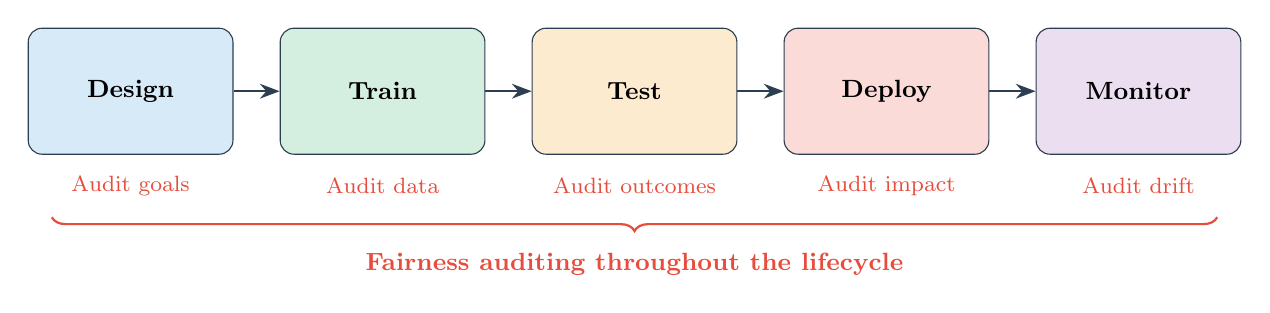
\begin{tikzpicture}[
    stage/.style={rectangle, rounded corners=5pt, draw=csprimary, fill=#1, minimum width=26mm, minimum height=16mm, font=\small\bfseries, align=center},
    arrow/.style={-{Stealth[length=2.5mm]}, thick, color=csprimary}
]

\node[stage=cstertiary!20] (design) at (0,0) {Design};
\node[stage=csaccent!20] (train) at (3.2,0) {Train};
\node[stage=cswarm!20] (test) at (6.4,0) {Test};
\node[stage=cssecondary!20] (deploy) at (9.6,0) {Deploy};
\node[stage=codepurple!20] (monitor) at (12.8,0) {Monitor};

\draw[arrow] (design) -- (train);
\draw[arrow] (train) -- (test);
\draw[arrow] (test) -- (deploy);
\draw[arrow] (deploy) -- (monitor);

% Audit points
\node[font=\footnotesize, color=cssecondary] at (0,-1.2) {Audit goals};
\node[font=\footnotesize, color=cssecondary] at (3.2,-1.2) {Audit data};
\node[font=\footnotesize, color=cssecondary] at (6.4,-1.2) {Audit outcomes};
\node[font=\footnotesize, color=cssecondary] at (9.6,-1.2) {Audit impact};
\node[font=\footnotesize, color=cssecondary] at (12.8,-1.2) {Audit drift};

\draw[decorate, decoration={brace, amplitude=5pt, mirror}, thick, cssecondary] 
    (-1,-1.6) -- (13.8,-1.6);
\node[font=\small\bfseries, color=cssecondary] at (6.4,-2.2) {Fairness auditing throughout the lifecycle};

\end{tikzpicture}
\end{center}

%---------- WHAT SHOULD WE DO ----------%
\section{What Should We Do?}

There are no easy answers to algorithmic fairness, but there are better and worse approaches. Here are principles that researchers and ethicists have proposed:

\textbf{Context matters.} The right definition of fairness depends on the domain. Equal accuracy might be paramount in criminal justice, where errors have severe consequences for individuals. Demographic parity might matter more in hiring, where we want to counteract historical exclusion.

\textbf{Humans should remain in the loop.} Algorithms can inform decisions, but humans should retain meaningful oversight, especially for high-stakes choices. A judge should consider a risk score as one input among many, not as a definitive answer.

\textbf{Affected communities should have voice.} People impacted by algorithmic systems should participate in decisions about how those systems are designed and deployed. Technical experts alone shouldn't decide what counts as ``fair.''

\textbf{We should measure and monitor.} You can't fix what you don't measure. Organizations deploying algorithms should continuously track outcomes across different groups and be prepared to adjust when problems emerge.

\textbf{Trade-offs should be explicit.} When perfect fairness is impossible, the choice of which fairness to prioritize should be made deliberately and transparently, not hidden in technical implementation details.

Ultimately, algorithms are tools created by humans, encoding human choices. They can perpetuate injustice or help remedy it---depending on how thoughtfully they're designed, deployed, and governed. As future programmers, you won't just write code; you'll make decisions that affect people's lives. Understanding these ethical dimensions is part of your professional responsibility.

%---------- DISCUSSION QUESTIONS ----------%
\section*{Discussion Questions}

\begin{questionbox}
\begin{enumerate}[leftmargin=*, label=\textcolor{cswarm}{\textbf{\arabic*.}}]
    \item \textbf{The Human Baseline:} Algorithms are often compared to an ideal of perfect fairness. But is the realistic alternative algorithmic decision-making or \textit{human} decision-making? Humans have biases too---studies show that identical résumés receive different responses depending on whether the name sounds white or Black, male or female. Does this change how we should evaluate algorithmic bias?

    \item \textbf{Choosing Fairness:} In the COMPAS case, ProPublica emphasized equal false positive rates (Black defendants were more often wrongly labeled high-risk), while Northpointe emphasized calibration (defendants with the same score had similar outcomes regardless of race). If you were a judge using such a system, which definition of fairness would matter more to you? Why?

    \item \textbf{The Proxy Problem:} If removing race from an algorithm's inputs doesn't prevent racially disparate outcomes (because of proxy variables like ZIP code), what should we do? Should we remove proxies too, even if they're genuinely predictive? Should we explicitly use race to counteract the proxies? What are the trade-offs?

    \item \textbf{Transparency vs.\ Gaming:} Making algorithms transparent allows auditing for fairness. But it also allows people to ``game'' the system---manipulating their inputs to get desired outcomes. How should we balance these concerns? Are there domains where transparency should be prioritized? Where it shouldn't?

    \item \textbf{Responsibility:} When an algorithm causes harm---say, wrongly denying someone a loan or keeping someone in jail who shouldn't have been---who is responsible? The programmers? The company? The organization that deployed it? The user who relied on it? How should we structure accountability for algorithmic systems?
\end{enumerate}
\end{questionbox}

%---------- GLOSSARY ----------%
\section*{Key Terms}

\begin{glossarybox}
\begin{description}[leftmargin=!, labelwidth=3.4cm, font=\bfseries\color{cssecondary}]
    \item[Algorithm] A precise sequence of steps for solving a problem, which can be executed automatically by a computer.
    
    \item[Algorithmic Auditing] Systematic testing of algorithms to detect bias, errors, or unintended consequences.
    
    \item[Algorithmic Fairness] The study of how to design algorithms that treat people equitably, encompassing multiple competing definitions.
    
    \item[Algorithmic Transparency] Making the logic, data, and decision processes of algorithms open to inspection and understanding.
    
    \item[Bias] Systematic errors or unfair preferences in algorithmic outputs, often reflecting historical discrimination in training data.
    
    \item[Black Box] A system whose internal workings are hidden or too complex to interpret, making decisions difficult to explain.
    
    \item[Demographic Parity] A fairness criterion requiring equal rates of positive outcomes across different demographic groups.
    
    \item[Equal Accuracy] A fairness criterion requiring equal error rates (false positives, false negatives) across groups.
    
    \item[Explainability] The degree to which a human can understand why an algorithm made a particular decision.
    
    \item[Individual Fairness] A fairness criterion requiring that similar individuals receive similar treatment.
    
    \item[Machine Learning] Algorithms that learn patterns from data rather than following explicitly programmed rules.
    
    \item[Proxy Variable] A variable that correlates with a protected characteristic (like race or gender) and can indirectly introduce bias.
    
    \item[Training Data] The historical examples used to teach a machine learning algorithm, which shape what patterns it learns.
\end{description}
\end{glossarybox}

\vspace{5mm}

%---------- FOOTER ----------%
\begin{center}
\textcolor{csprimary}{\rule{0.6\textwidth}{0.5pt}}\\[3mm]
{\small\textcolor{gray}{This case study is part of the Open Educational Resources for \cscourse.\\
Licensed under Creative Commons Attribution 4.0 (CC BY 4.0).}}
\end{center}

\end{document}